
% ==================================================
%	Theorie
% ==================================================

\section{Theorie}

Das Rauschen stellt einen statistischen Prozess dar. Dabei ist weicht ein
Signal gleichverteilt mit sehr kleinen Schwankungen um einen Mittelwert ab.
Folglich ist das zeitliche Mittel bei einem hinreichend großen
Integrationsintervall gleich null.
Somit wird, um das Rauschen dennoch untersuchen zu können, das Quadrat des
Rauscheffekts verwandt.
Bei einem Zeitintervall von $\tau_0$ bist $\tau$ wird somit
\begin{equation}
  \overline{U^2(t)} \coloneqq \frac{1}{\tau} \int_{\tau_0}^{\tau} U^2(t) \dd{t}
\end{equation}
betrachtet.
Wenn dieser Mittelwert unabhängig von der Wahl des Zeitintervalls ist, so wird
die Schwankungserscheinung \emph{stationär} bezeichnet.
Das quadratische Mittel lässt sich zudem auch aus dem \emph{Scharmittel}
bestimmen. Hierbei wird eine große Anzahl von identischen Rauschquellen zu
einem Zeitpunkt $t_0$ betrachtet, wobei die Spannungswerte $U_i(t_0)$
aufgenommen werden.
Das Scharmittel wird dann entsprechend
\begin{equation}
  \ev{U^2(t_0)} \coloneqq \frac{1}{N} \sum_{i=1}^N U_i^2(t_0)
\end{equation}
ermittelt.
In diesem Fall ist die Schwankungserscheinung stationär, wenn das Scharmittel
unabhängig vom Zeitpunkt $t_0$ ist.
Stimmen das Scharmittel und das zeitliche Mittel überein, so wird die
Schwankungserscheinung \emph{ergodisch} bezeichnet.
Die in diesem Versuch betrachteten Rauscheffekte lassen sich dabei alle zu den
ergodischen Prozessen einordnen.

% ==================================================
% 	Thermisches Rauschen
% ==================================================

\subsection{Thermisches Rauschen}
\label{sub:thermisches_rauschen}

\begin{figure}[!htpb]
  \centering
  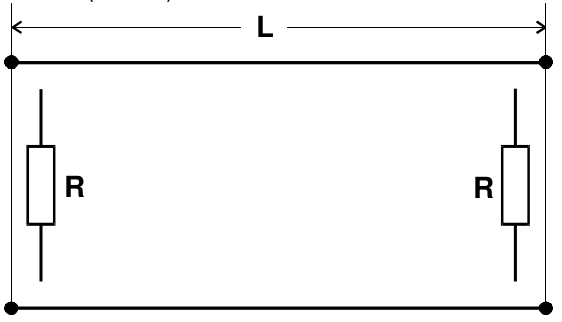
\includegraphics[scale=0.3]{bilder/doppelleitung.png}
  \caption{Darstellung einer parallelen, verlustlosen Doppelleitung.\cite{FP}}
\label{fig:doppelleitung}
\end{figure}

Die Schwankungen aus Abbildung~\ref{fig:rauschen} an den Enden eines ohmschen
Widerstands lassen sich durch das Phänomen des thermischen Rauschens erklären.
Die Spannung $U(t)$ entsteht dabei durch die ungeordnete Wärmebewegung der
Elektronen. So verschiebt sich der Ladungsschwerpunkt für eine kurze Zeit näher
an ein Ende des Widerstands, sodass dieses Ende gegenüber zu dem anderen Ende
ein negatives Potential aufweist.
Im Folgenden soll die Herleitung der \textsc{Nyquist}-Beziehung, welche eine
Beziehung zwischen dem Rauschspannungsquadrat und der Temperatur herstellt,
gezeigt werden.

Hierzu wird eine Doppelleitung, wie in Abbildung~\ref{fig:doppelleitung}
gezeigt, betrachtet. Zunächst seien die Enden der Leitungen kurzgeschlossen.
Dieses System ist schwingfähig, wobei Schwingungen der Wellenlänge
\begin{equation}
  L = n \frac{\lambda}{2}
\end{equation}
möglich sind.
Betrachtet man die Phasengeschwindigkeit $v$ und die Frequenz $\nu$ der
Schwingungen, so ist die Anzahl $\Delta n$ der Eigenschwingungen im
Frequenzintervall $\nu$ bis $\nu + \Delta \nu$
\begin{equation}
  \Delta n = \frac{2L}{v} \Delta \nu~.
  \label{eq:eigenschwingung}
\end{equation}
Für $L \gg \lambda$ ist~\eqref{eq:eigenschwingung} ein quasikontinuierlich.
Angenommen das System befindet sich im thermodynamischen Gleichgewicht, dann
gilt der Gleichverteilungsatz der Thermodynamik, worin jede Schwingung die
mittlere Frequenz
\begin{equation}
  \overline{E} = \frac{\text{h}\nu}{\exp[\frac{\text{h}\nu}{k_\text{B}T}] - 1}
\end{equation}
besitzt.
Somit ist der mittlere Energiegehalt in den Frequenzintervall $\Delta \nu$
\begin{equation}
  \Delta n \overline{E} =
  \frac{2L}{v}
  \frac{\text{h}\nu}{\exp[\frac{\text{h}\nu}{k_\text{B}T}] - 1} \Delta \nu~.
  \label{eq:mittlerer_energiegehalt}
\end{equation}
Die stehenden Wellen in der Leitung können jedoch als Superposition zweier
gegenläufigen Wellen betrachtet werden. Daher kann die Energie (die Hälfte von
\eqref{eq:mittlerer_energiegehalt}), welche in
einer Richtung durch die Leitung in einem Umlauf transportiert wird, durch
die Leistung
\begin{equation}
  P = \frac{\text{h}\nu}{\exp[\frac{\text{h}\nu}{k_\text{B}T}] - 1} \Delta \nu~.
  \label{eq:leistung}
\end{equation}
beschrieben werden, da die Zeit für einen Umlauf hier $L/v$ beträgt.

Ersetzt man nun den Kurzschluss der beiden Enden durch zwei Widerstände,
so wird an den Widerständen die Leistung~\eqref{eq:leistung} in Wärme
umgesetzt.
Da sich das System im Thermodynamik Gleichgewicht befindet, muss diese Leistung
dem System wieder hinzugefügt werden.
Dies geschieht in Form einer elektrischen Leistung, sodass die Widerstände
eine Rauschspannung $U_R(t)$ erzeugen.
Die mittlere Rauschleistung beträgt dabei
\begin{equation}
  \overline{P} = Z \overline{I^2} = \overline{U^2} \frac{Z}{{(R+Z)}^2}~,
\end{equation}
mit der mittleren Rauschspannung $\overline{U^2}$, dem mittleren Rasuchstrom
$\overline{I^2}$ und dem Wellenwiderstand $Z$.
Hierbei ist die Leistung maximal bei $Z=R$ und somit bei
\begin{equation}
  \overline{P}_\text{max} = \frac{\overline{U^2}}{4R}~.
\end{equation}
Hiermit und mit der Gleichung~\eqref{eq:leistung} erhält man schließlich eine
Beziehung zwischen dem Rauschspannungsquadrat und der Temperatur gemäß
\begin{equation}
  \overline{U^2}(\nu) = 4RP = 4R
  \frac{\text{h}\nu}{\exp[\frac{\text{h}\nu}{k_\text{B}T}] - 1} \Delta \nu~.
\end{equation}
Der Verlauf der Kurve ist in Abbildung~\ref{fig:spannungsquadrat} dargestellt.
Hierin ist zu erkennen, dass im elektronischen Frequenzbereich von bis zu
\SI{10^{12}}{\hertz} praktisch nicht
von $\nu$ abhängt. Somit kann für $\text{h}\nu \gg k_\text{B}T$ die Näherung
\begin{equation}
  \exp[\frac{\text{h}\nu}{k_\text{B}T}] = 1 + \frac{\text{h} \nu}{k_\text{B}T}
  + \ldots
\end{equation}
die sogenannte \textsc{Nyquist}-Beziehung angegeben werden mit
\begin{equation}
  \overline{U^2} = 4 k_\text{B} T R \Delta \nu~.
  \label{eq:nyquist}
\end{equation}
Hieran ist zu erkennen, dass $\overline{U^2}$ nur noch von der Breite des
betrachteten Frequenzbandes abhängig ist.

\begin{figure}[!htpb]
  \centering
  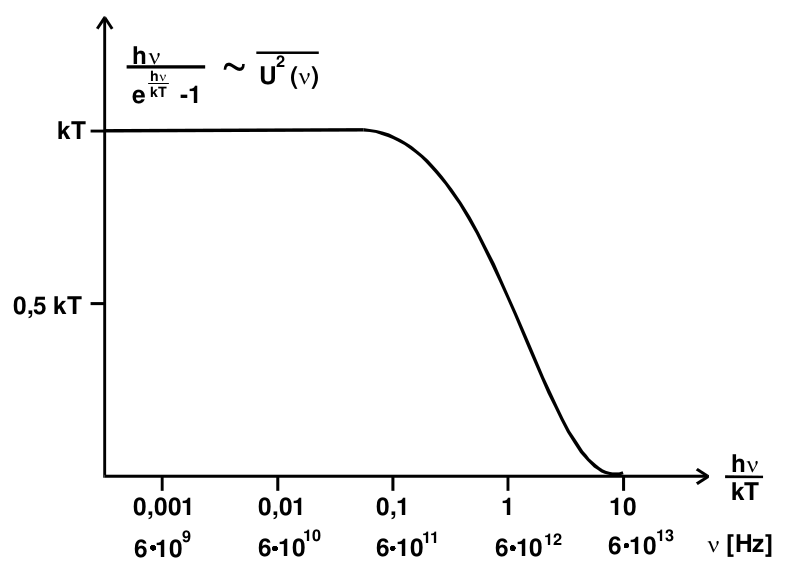
\includegraphics[scale=0.3]{bilder/spannungsquadrat.png}
  \caption{Frequenzabhängigkeit der Rauschspannung an einem ohmschen
    Widerstand.\cite{FP}}
\label{fig:spannungsquadrat}
\end{figure}

\paragraph{Realer Widerstand}
\label{par:realer_widerstand}

Bei der Vermessung des Rauschens eines Widerstandes ist zu beachten, dass ein
realer Widerstand neben dem ohmschen Widerstand im Ersatzschaltbild auch eine
parallelen kapazitiven Anteil besitzt.
Dadurch wird das messbare Rauschspannungsquadrat $\overline{U_\text{RC}^2}$
verringert gemäß
\begin{equation}
  \overline{U_\text{RC}^2} = \overline{U_R^2} \frac{1}{1 + {(2\pi\nu RC)}^2}~.
\end{equation}
Hierin ist $\overline{U_R}^2$ das theoretisch vorhergesagte
Rauschspannungsquadrat.

% ==================================================
% 	Schrotrauschen
% ==================================================

\subsection{Schrotrauschen}
\label{sub:schrotrauschen}

Die Emission von Elektronen aus Festkörperoberflächen stellt ebenfalls einen
statistischen Prozess dar, da die emittierten Elektronen aufgrund ihrer
endlichen Größe Zufallsschwankungen unterworfen sind.
Somit ist der Strom eine Hochvakuumdiode nicht konstant und nimmt beispielhaft
eine Form wie in Abbildung~\ref{fig:diodenstrom} an.
Das Auftreffen der Elektronen auf die Anode ähnelt dem Auftreffen von
Schrotkörnern auf eine Metallplatte, weshalb dieser Rauscheffekt als
\emph{Schroteffekt} bezeichnet wird.

\begin{figure}[!htpb]
  \centering
  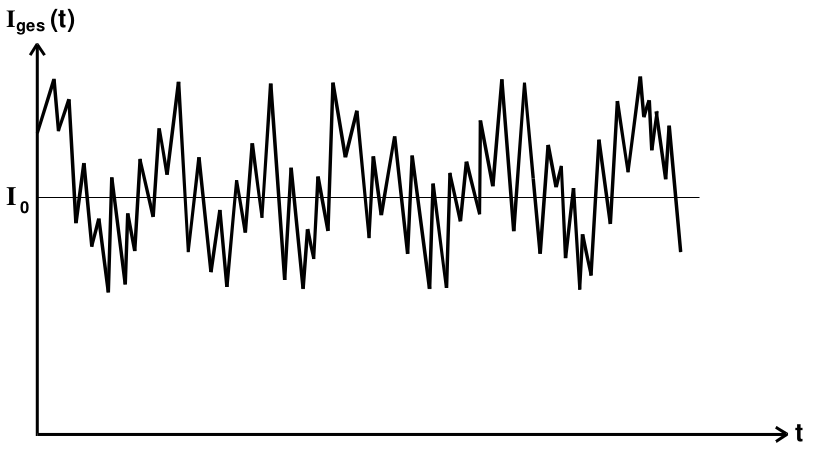
\includegraphics[scale=0.3]{bilder/diodenstrom.png}
  \caption{Zeitlicher Verlauf des Anodenstrom in einer
    Hochvakuumdiode.\cite{FP}}
\label{fig:diodenstrom}
\end{figure}

\begin{figure}[!htpb]
  \centering
  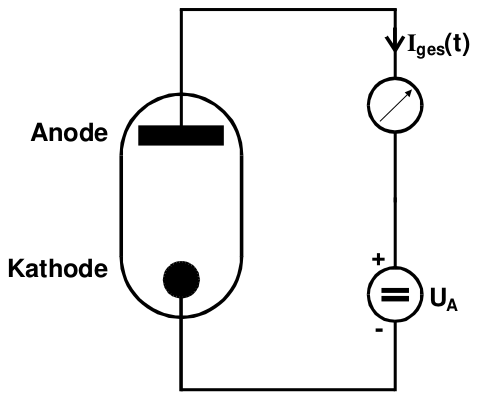
\includegraphics[scale=0.3]{bilder/diode.png}
  \caption{Aufbau einer Vakuumdiode zur Messung des Schrotrauschens.\cite{FP}}
\label{fig:diode}
\end{figure}

Der Schroteffekt lässt sich am besten an einer Hochvakuumdiode mit einer
Reinmetallkathode im Sättigungsbereich studieren.
Der prinzipielle Aufbau der Messung des Schrotrauschens ist in
Abbildung~\ref{fig:diode} dargestellt.
Hierbei kann der Gesamtstrom $I_\text{ges}$ durch einen Gleichstromanteil $I_0$
und einen Wechelstromanteil $I(t)$, welcher den Rauschanteil darstellt,
beschrieben werden gemäß
\begin{equation}
  I_\text{ges} (t) = I_0 + I(t)~.
\end{equation}
Für den mittleren Rauschstrom gilt analog zum thermischen Rauschen
$\overline{I(t)} = 0$, sodass wieder das Quadrat des Rauscheffekts, in diesem
Fall das Rauschstromquadrat $\overline{I^2}$, betrachtet wird.
Zur Bestimmung des Rauschstromquadrats werden folgende Annahmen gemacht:
\begin{enumerate}
  \item Die Elektronen werden unabhängig voneinander emittiert.
  \item Die Elektronen sind unabhängig von deren Weschelwirkungen
    untereinander.
  \item Die Elektronen starten mit Anfangsgeschwindigkeit null.
  \item Alle Elektronen zeigen den gleichen Weg-Zeit-Verlauf.
  \item An der Anode entstehen keine Sekundärelektronen.
\end{enumerate}

Im Folgenden soll nun ein Ausdruck für das Rauschstromsquadrat hergeleitet
werden.
Dabei wird zunächst das Verhalten eines \emph{einzelnen} Elektrons beim
Durchlauf der Diode betrachtet werden.
Der Stromimpuls dieses Elektrons ist gegeben durch%
\begin{equation}
  i_n(t) = \e_0 f(t - t_n)~,
\end{equation}
wobei die Funktion $f(t)$ die Form des Stromimpulses $i(t)$ beschreibt und für
alle Elektronen gleich ist.
Zudem ist sie nur für einen Zeitraum $\tau$ von null
verschieden und beginnt bei dem $n$-ten Elektron zum Zeitpunkt $t_n$.
Der Anodenstrom, der durch alle Elektronen erzeugt wird ist somit
\begin{equation}
  I_\text{ges}(t) = \e_0 \sum_n f(t-t_n)~.
\end{equation}
Nun gilt für die Mittelwerte der Ströme
\begin{equation}
  I_0 = \overline{I_\text{ges}}\qquad \text{und} \qquad
  \overline{I(t)} = 0~,
\end{equation}
sodass für das quadratischen Mittel
\begin{equation}
  \overline{I_\text{ges}^2} = I_0^2 + \overline{I^2(t)}
\end{equation}
folgt.
Aufgrund der statistischen Unabhängigkeit der Elektronen lässt sich der
Gesamteffekt des Rauschen mit Hilfe des \textsc{Campbell}'schen Theorems
als Summe aus den quadratischen Beiträgen der einzelnen Elektronen beschreiben.
Dies liefert mit der Impulsdichte $z$ (Anzahl von Impulsen pro Sekunde)
\begin{equation}
  I_0 = z \int_{0}^{\tau} \e_0 f(t) \dd{t} = z\e_0
\end{equation}
und
\begin{equation}
  \overline{I^2(t)} = z \int_{0}^{\tau} \e_0^2 f^2(t) \dd{t}~.
  \label{eq:rauschstrom_zeit}
\end{equation}
Ist nun $f(t)$ bekannt, so lässt sich das quadratische Mittel des
Rauschstroms bestimmen.
Nun ist es zudem interessant das Rauschspektrum $W_\text{Sch}$
zu betrachten. Dies ist definiert über
\begin{equation}
  \overline{I^2(t)} = \int_{0}^{\infty} W_\text{Sch}(\nu) \dd{\nu}~.
  \label{eq:rauschspektrum}
\end{equation}
Zur Berechnung von $W_\text{Sch}{\nu}$ wird die \textsc{Fourier}-transformierte
$F(\nu)$ von $f(\tau)$ betrachtet. Hier gilt letztendlich mit Hilfe des
\textsc{Parseval}'schen Theorems
\begin{equation}
  \int_{0}^{\tau} f^2(t) \dd{t} = \int_{0}^{\infty} {\abs{F(\nu)}}^2 \dd{\nu}~.
\end{equation}
Somit folgt für den Rauschstrom aus~\eqref{eq:rauschstrom_zeit}
\begin{equation}
  \overline{I^2} = 2\e_0 I_0 \int_{0}^{\infty} {\abs{F(\nu)}}^2 \dd{\nu}
\end{equation}
und im Vergleich mit~\eqref{eq:rauschspektrum}
\begin{equation}
  W_\text{Sch} = 2 \e_0 I_0 {\abs{F(\nu)}}^2~.
\end{equation}
Für den Bereich niedriger Frequenzen $\nu \ll 1/(2\pi\tau)$ gilt
$F(\nu) \approx 1$ und somit vereinfacht sich das Rauschspektrum zu
\begin{equation}
  W_\text{Sch}(\nu) = 2 \e_0 I_0
\end{equation}
und ist somit frequenzunabhängig und stellt für Frequenzen unterhalb
\SI{100}{\mega\hertz} eine gute Näherung dar.
Der Vergleich mit Gleichung~\eqref{eq:rauschspektrum} ergibt nun die
sogenannte \textsc{Schottky}-Beziehung
\begin{equation}
  \overline{I^2} = 2 \e_0 I_0 \Delta \nu~,
\end{equation}
wobei $\Delta\nu$ den Frequenzbereich darstellt indem $\overline{I^2}$
gemessen wird.

% ==================================================
% 	1/f Rauschen
% ==================================================

\subsection{$1/f$-Rauschen}
\label{sub:_1_f_rauschen}

Die spektrale Leistungsdichte von Rauschprozesse gehorchen einer
$1/\nu$-Gesetzmäßigkeit. Diese Beobachtung ist rein phänomenologisch, sodass es
noch keine umfassende Theorie zu Beschreibung dieses Phänomens gibt.
Diese $1/\nu$-Gesetzmäßigkeit beschränkt sich dabei nicht nur auf elektronische
Bauelemente wie z.B. Widerständen, Halbleiterbauelemente und Elektronenröhren,
sondern man findet sie auch bei astronomischen, meteorologischen oder
physiologischen Bereichen.
Diese Gesetztmäßigkeit erstreckt sich dabei über mehrere Zehnerpotenzen und es
kann keine untere Schranke angegeben werden.

Nun gibt es einige Spezialfälle in denen die $1/\nu$-Gesetzmäßigkeit abgeleitet
werden kann. Ein solcher Spezialfall ist das
\emph{Generations-Rekombinations-Rauschen}. Dies betrifft die Generations und
Rekombinationsvorgänge von Ladungsträgern in Oxid-Halbleiter-Grenzschichten,
wie beispielsweise von MOS-Feldeffekttransistoren.
Die spektrale Leistungsdichte der Dichteschwankungen der Ladungsträger lautet
hier
\begin{equation}
  W_\tau(\nu) = \text{const} \cdot \frac{\tau}{1 + {(2\pi\nu\tau)}^2}~,
  \label{eq:leistungsdichte}
\end{equation}
wobei $\tau$ die Relaxationszeit für den Generations-Rekombinationseffekt ist.
Für $\nu \ll 1 / \tau$ ist~\eqref{eq:leistungsdichte} nahezu konstant.
Erst für $\nu > 1 / \tau$ fällt $W$ zunehmend ab.
Diese Kurve ist in Abbildung~\ref{fig:leistungsdichte} dargestellt.

\begin{figure}[!htpb]
  \centering
  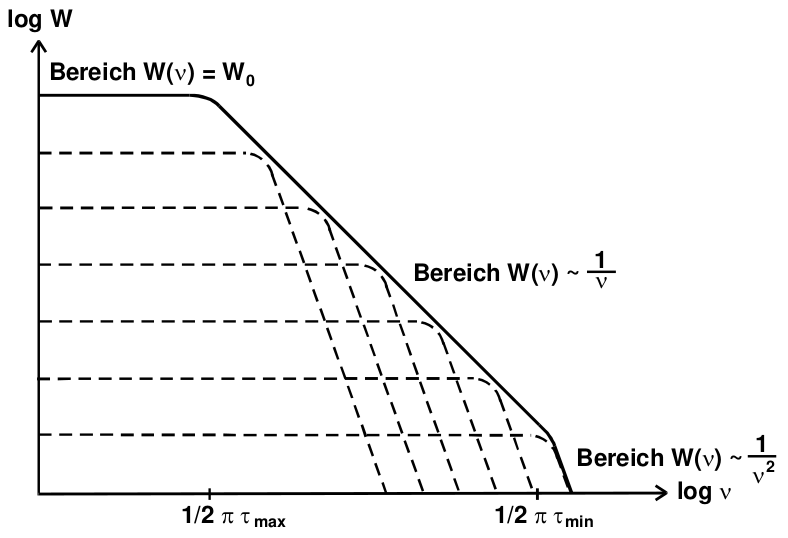
\includegraphics[scale=0.3]{bilder/leistungsdichte.png}
  \caption{Modell-Rauschspektrum zur Ableitung einer Beziehung von der Gestalt
  $W(\nu)\sim\nu^{-1}$.\cite{FP}}
\label{fig:leistungsdichte}
\end{figure}

Nimmt man nun $\tau$ nicht mehr als konstant an, sondern abhängig von der
Aktivierungsenergie $E$, welche zwischen den Werten $E_\text{min}$ und
$E_\text{max}$ liegt mit
\begin{equation}
  \tau(E) = \tau_0 \exp[\frac{E}{k_\text{B}T}]~,
\end{equation}
so folgt für das Gesamtspektrum
\begin{equation}
  W(\nu) = \text{const} \cdot k_\text{B} T
  \int_{\tau_\text{min}}^{\tau_\text{max}}
  \frac{1}{1 + {(2\pi\nu\tau)}^2} \dd{\tau}
  = \frac{\text{const} \cdot k_\text{B}T}{\nu}
  \qty\Big(\arctan(2\pi\nu\tau_\text{min}) - \arctan(2\pi\nu\tau_\text{max}))~.
\end{equation}
Hier können nun drei Frequenzbereiche aus Abbildung~\ref{fig:leistungsdichte}
beschrieben werden:
\begin{enumerate}
  \item Für sehr niedrige Frequenzen ist $2\pi\nu\tau \ll 1/\tau$ und
    $W(\nu) = \text{const}$. Es handelt sich um weißes Rauschen.
  \item Für $2\pi\nu \tau_\text{min} \ll 1 \ll 2\pi\nu\tau_\text{max}$ liegt
    eine $1/\nu$-Abhängigkeit der spektralen Leistungsdichte vor.
  \item Für sehr hohe Frequenzen $2\pi\nu\tau \gg 1$ liegt eine
    $1/\nu^2$-Abhängigkeit der spektralen Leistungsdichte vor.
\end{enumerate}

% ==================================================
% 	Funkeleffekt
% ==================================================

\subsection{Funkeleffekt}
\label{sub:funkeleffekt}

In diesem Versuch soll der sogenannte Funkeleffekt untersucht werden.
Dieser ist ein Beispiel für das $1/f$-Rauschen.
Er tritt bei Elektronenröhren mit Oxid-Kathode auf. Hierbei ist dem weißen
Rauschen des Schrot-Rauschens ein weiterer Rauscheffekt überlagert dessen
Frequenzspektrum die Form
\begin{equation}
  W_F(\nu) = \text{const} \cdot \frac{{I_0}^2}{\nu^\alpha}
\end{equation}
mit $\alpha \approx 1$ besitzt.
Diese Form konnte bis zu Frequenzen von \SI{0.1}{\milli\hertz} experimentell
bestätigt werden.
Für den unteren Frequenbereich könnten dabei stoffliche Veränderungen in dem
System Metallträger-Oxid-Kathode infrage kommen.
Bei höheren Frequenzen könnten lokale Schwankungen der Austrittsarbeit des
Oxidmetalls den Rauscheffekt erklären, wobei vorübergehende Fremdatome an der
Oberfläche absorbiert werden.
